\documentclass[fontset=windows]{article}
\PassOptionsToPackage{quiet}{xeCJK}
\usepackage{lshort-zh-cn-style}
\usepackage{My}
\usetikzlibrary{arrows.meta}    % 画箭头用的包



\begin{document}
\begin{center}
\tableofcontents
\end{center}
\newpage

\section{函数绘制}
\subsection{绘制二维函数图像}
\begin{figure}[!htb]
    \begin{minipage}[t]{0.5\linewidth}
    \vspace*{0pt}
    如下图,绘制函数图像
    
    \vspace*{1cm}
    \noindent$
    \begin{aligned}
        & y = 2x^2-1\\
        &y = x\\
        & y = \sin(x)\\
        &y = e^x  \\ 
        & \left \{ \begin{matrix} x = 2.5\sin(t)\\ y = 1.5\cos(t)\end{matrix}\right.      
    \end{aligned}
    $ 
    \end{minipage}
    \begin{minipage}[t]{0.5\linewidth}
        \vspace*{0pt}
        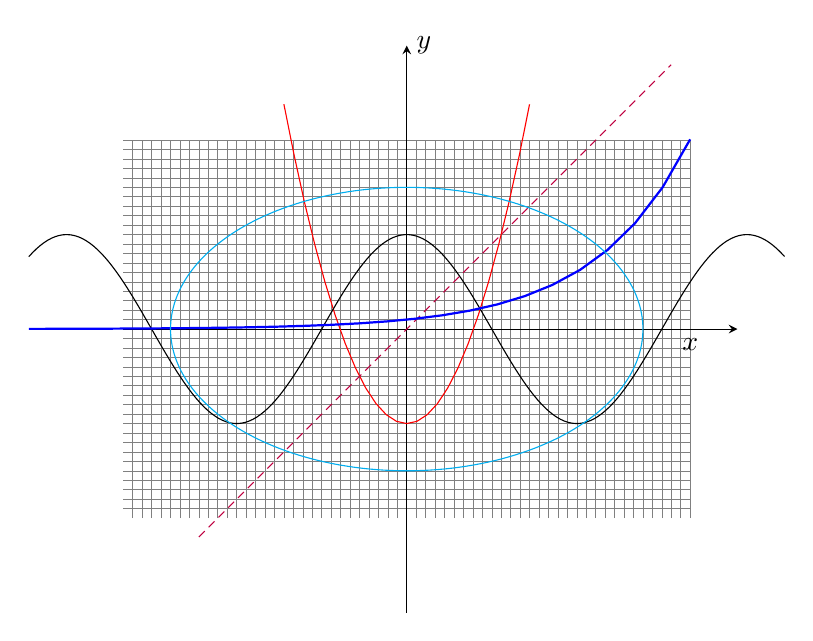
\begin{tikzpicture}[scale=1.2]
            \draw[help lines,step=0.1]
            (-3,-2) grid (3,2);
            % 使用node不方便控制,所以使用coordinate更加的方便
            \draw[-stealth] (-3,0) -- (3.5,0);
            \coordinate[label=right:{$y$}] (y-axis) at (0,3);
            % \node (x) at (3,-0.1) {$x$};      
            \draw[-stealth] (0,-3) -- (0,3);
            \coordinate[label=below:{$x$}] (x-axis) at (3, 0);
            % \node (x) at (0.1, 3) {$y$};
            \draw[domain=-1.3:1.3, red]
                plot(\x, {\x*\x*2 -1});
            \draw[domain=-4:4][samples = 200]       % sample控制描点的个数,使得曲线更加的光滑
                plot(\x, {cos(100*\x)});
            \draw[domain=-2.2:2.8, color=purple, densely dashed][samples = 200]
                plot(\x, {\x});
            \draw[domain=-4:3, color=blue, thick]
                plot(\x, {0.1*exp(\x)});
            % 2. 使用参数方程绘图
            \draw[domain = -2:360, color=cyan][samples = 200] plot({2.5*sin(\x)},{1.5*cos(\x)});
            % 3. Vscode 内置的方式
        \end{tikzpicture}           
    \end{minipage}
\end{figure}

% 自定义函数: binom function
\vspace*{-3em}
\subsection{自定义函数}
\begin{example}
\tikzset{
    declare function={
    binom(\k,\n,\p)=
        \n!/(\k!*(\n-\k)!)*\p^\k*(1-\p)^(\n-\k);
        }
    }
\begin{tikzpicture}[scale=0.7]
    \begin{axis}[samples at={0,...,40},
            yticklabel style={
            /pgf/number format/fixed,
            /pgf/number format/fixed zerofill,
            /pgf/number format/precision=2}
        ]
    \addplot [only marks,orange] {binom(x,40,0.5)};
    \addlegendentry{$p=0.5$}
    \addplot [only marks,cyan] {binom(x,40,0.2)};
    \addlegendentry{$p=0.2$}
    \addplot [smooth,thick,cyan] {binom(x,40,0.2)};
    \addlegendentry{$p=0.2$}
    \end{axis}
\end{tikzpicture}     
\end{example}

\begin{itemize}
	\item help lines:显示背景网格辅助线
	\item step:domain区间内step参数控制网格大小
	\item domain:函数的绘制区间
\end{itemize}


\subsection{使用自定义的坐标轴绘图}
\begin{example}
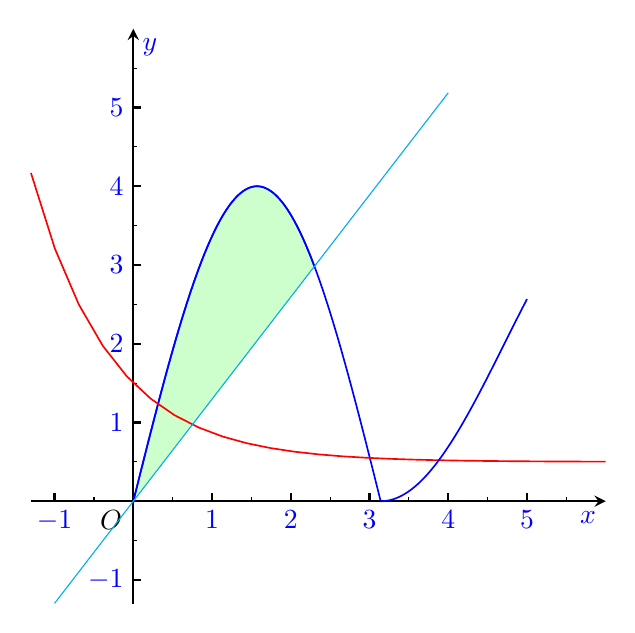
\begin{tikzpicture}{smooth}
% 1. 标记重要的点
\coordinate (O) at (0, 0);
\coordinate (ymax) at (0, 6);
\coordinate (ymin) at (0, -1.3);
\coordinate (xmax) at (6, 0);
\coordinate (xmin) at (-1.3, 0);

% 2. 绘制基本的坐标轴
\draw[-stealth, thick] (ymin) -- (ymax);
\draw[-stealth, thick] (xmin) -- (xmax);
\node[blue, right=6pt, below] at (ymax) {$y$};
\node[blue, below=6pt, left] at (xmax) {$x$};

% 3. 给x, y轴加上刻度
\node[black, left=8pt, below] at (O) {$O$};
\draw[black] (0, 0.5) -- (0.05, 0.5);
\draw[black] (0.5, 0) -- ( 0.5, 0.05);
\foreach \loc/\x in
    {-1/-1, 1/1, 2/2, 3/3, 4/4, 5/5}
    {\node[blue, below] at (\loc, 0) {$\x$};
     \draw[black, thick] (\loc, 0) -- (\loc, 0.1);
     \draw[black] (\loc+0.5, 0) -- (\loc+0.5, 0.05);
    } 
\foreach \loc/\y in
    {-1/-1, 1/1, 2/2, 3/3, 4/4, 5/5}
    {\node[blue, left] at (0, \loc) {$\y$};
     \draw[black, thick] (0, \loc) -- (0.1, \loc);
     \draw[black] (0, \loc+0.5) -- (0.05, \loc+0.5);
    } 
% 4. 绘制函数图
% 使用deg让它认识弧度制
\draw[blue, semithick, domain=0:2.3, fill=green!20][samples=200] plot (\x, {4*sin(deg(\x))});
\draw[blue, semithick, domain=0:pi][samples=200] plot (\x, {4*sin(deg(\x))});
\draw[red, semithick,  domain=-1.3:6] plot(\x, {exp(-\x)+0.5});
\draw[cyan, domain=-1:4] plot(\x,{4*sin(deg(2.3))/2.3*\x});
\draw[blue, semithick, domain=pi:5][samples=200] plot (\x, {2*sin(deg(\x + pi/2))+2});
% \draw [domain=0:1.7, black] (1.7, sin(deg(1.7))) -- (1.7, 0);
% \draw [fill =green!30] 
\end{tikzpicture}
\end{example}

\subsection{函数阴影的填充}
\begin{example}
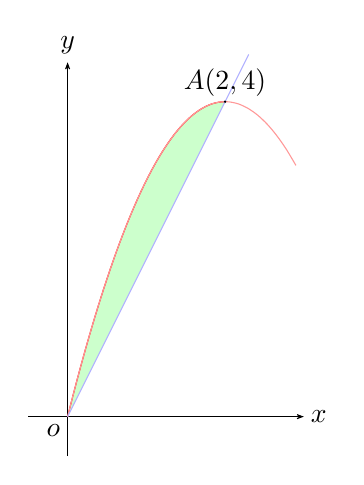
\begin{tikzpicture}[smooth]
    \draw[arrows={-Stealth[length=5pt, inset=3.5pt]}] 
        (-0.5,0) -- (3.0,0)
        node (xaxis) [right=-1pt] {$x$};
    \draw[arrows={-Stealth[length=5pt, inset=3.5pt]}] 
        (0,-0.5) -- (0,4.5)
        node (yaxis) [above=-0.6pt] {$y$};
    \draw  (-0.18,-0.18) node {$o$};
    \draw[color=red,domain=0:2.0,fill=green!20] 
        plot (\x,4*\x-\x*\x);
    \draw[color=red!40,domain=0:2.90] 
        plot (\x,4*\x-\x*\x)  ;
    \draw[color=blue!30,domain=0:2.3] 
        plot (\x,2*\x)  ;
    \draw[fill=black] 
        (2,4) circle [radius=0.2pt] 
        node[above=-1.8pt] {$A(2,4)$};
\end{tikzpicture}
\end{example}


\subsection{封装绘图函数框架}
% 注意:自定义命令中没有前后前后定义的,但是自定义环境有
% \newenvironment{}[][]{}{}
% \newcommand{}[][]{}

\begin{Axis}
    \draw[color=red,domain=0:2.0,fill=green!20] 
        plot (\x, {4*\x-\x*\x});
    \draw[color=blue!30,domain=0:2.3] 
        plot (\x,{ 2*\x});
    \draw[color=black,domain=-1.5:5] 
        plot (\x,{exp(-\x)});  
\end{Axis}
\begin{minipage}[t]{0.5\linewidth}
    \begin{Axis}
        \draw[color=red,domain=1:4.5,fill=blue!20] 
            plot (\x, {4*sin(0.5*\x r)});
        \draw[color=red, thick, domain=-1:4.5] 
            plot (\x,{4.5*(1-\x/4)});
    \end{Axis}
\end{minipage}


\section{内置绘图命令}
\subsection{数据绘图}
%% 从数据文件读取数据绘图
\begin{center}
\begin{tikzpicture}
	\begin{axis}
	\addplot3[surf,mesh/ordering=y varies]
	table {./data/concat_VV_together.dat};
	\end{axis}
\end{tikzpicture}
\end{center}

\subsection{三维曲面绘制}
\begin{figure}[!htb]
    \begin{minipage}[t]{.33\linewidth}
    {\bf mesh}
	 %% mesh
		\begin{tikzpicture}[scale=.7]
			 \begin{axis}[title = 我是title,
			    			hide axis,		%% 隐藏坐标轴
			    			colormap/cool	%% 指定色系
			    ]\addplot3[mesh, samples=50, domain=-8:8]{x*y/(x^2+y^2)};
		        \addlegendentry{$\frac{\sin(r)}{r}$}	%% 添加图例
		    \end{axis}
		\end{tikzpicture}
    \end{minipage}
    \vline
    \begin{minipage}[t]{.33\linewidth}
    {{\bf default}}
    %% 默认方法
        \begin{tikzpicture}[scale=.7]
		    \begin{axis}[title = 我是title,
		    	     		hide axis,		%% 隐藏坐标轴
		    				colormap/cool	%% 指定色系
		    	 ]
		        \addplot3[samples=50, domain=-8:8]{sin(deg(sqrt(x^2+y^2)))/sqrt(x^2+y^2)};
		        \addlegendentry{$\frac{\sin(r)}{r}$}	%% 添加图例
		    \end{axis}
		\end{tikzpicture}
    \end{minipage}
    \vline
    \begin{minipage}[t]{.33\linewidth}
    {\bf surf}
    %% surf方法
        \plotz{scale=.75}{sin(deg(sqrt(x^2+y^2)))/sqrt(x^2+y^2)}{surf}{}{图例}
    \end{minipage}
\end{figure}

\subsection{TikZ中旋转与平移}
\begin{figure}[!htb]
    \begin{minipage}[t]{.5\linewidth}
    \centering
      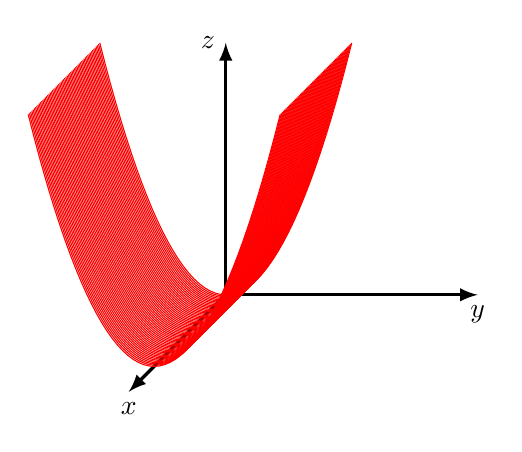
\begin{tikzpicture}[scale=.8]
			\coordinate (O) at (0,0,0);
			\draw[very thick, ->, >=latex] (O) -- (4,0,0) node[below]{\(y\)};
			\draw[very thick, ->, >=latex] (O) -- (0,4,0) node[left]{\(z\)};
			\draw[very thick, ->, >=latex] (O) -- (0,0,4) node[below]{\(x\)};
			
			\foreach \z in {0,0.05, ..., 3}{
				\draw[red, domain=0:2] plot (\x,\x*\x,\z);
				\draw[red, domain=0:2] plot (-\x,\x*\x,\z);
			}
		\end{tikzpicture}
    \end{minipage}
    \vline
    \begin{minipage}[t]{.5\linewidth}
    \centering
       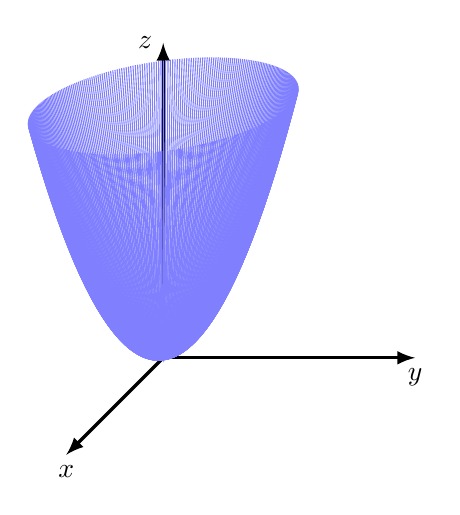
\begin{tikzpicture}[scale=.8]
			\coordinate (O) at (0,0,0);
			\draw[very thick, ->, >=latex] (O) -- (4,0,0) node[below]{\(y\)};
			\draw[very thick, ->, >=latex] (O) -- (0,5,0) node[left]{\(z\)};
			\draw[very thick, ->, >=latex] (O) -- (0,0,4) node[below]{\(x\)};
			
			\foreach \angle in {0, ..., 360}{
				\draw[blue!50, rotate around y=\angle, domain=0:2] plot (\x,\x*\x, 0);
			}
		\end{tikzpicture}
    \end{minipage}
\end{figure}

\section{命令封装}
\subsection{极坐标图形绘制}
\begin{figure}[!htb]
    \begin{minipage}[t]{.33\linewidth}
    \centering
       \begin{Plot}{scale=0.8}{>=stealth}
			\plot{blue!40, thick}{-1:3}{\x*\x-2*\x-1}
			\plot{red, thick}{0:pi}{3*sin(\x r)}
		\end{Plot}
    \end{minipage}
    \begin{minipage}[t]{.33\linewidth}
    \centering
        \polarplot{scale=0.2}{cyan, domain=0:1440}{0.02/pi*\t}
    \end{minipage}
    \begin{minipage}[t]{.33\linewidth}
    \centering
        \polarplot{scale=2}{red, domain=0:720}{sin(2*\t)}
    \end{minipage}
\end{figure}

\subsection{二维参数方程}
\begin{figure}[!htb]
    \begin{minipage}[t]{.5\linewidth}
    \centering
		\paraplot{scale=1}{{3*cos(t)}, {sin(t)}}{thick, color=blue}{hide axis}
    \end{minipage}
    \begin{minipage}[t]{.5\linewidth}
    \centering
        \paraplot{scale=1}{{1.3*cos(t)}, {1.3*sin(t)}}{thick, color=blue}{hide axis}
    \end{minipage}
\end{figure}

\subsection{三维参数方程}
\begin{figure}[!htb]
    \begin{minipage}[t]{.33\linewidth}
    \centering
        \paraplotz{scale=0.5} {{sin(deg(t))},{cos(deg(t))},{t}} {}{view = {60}{90}, hide axis}
    \end{minipage}
    \begin{minipage}[t]{.33\linewidth}
        \paraplotz{scale=0.5}{{sin(deg(t))},{cos(deg(t))},{t}}{}{view = {90}{30}}
    \end{minipage}
    \begin{minipage}[t]{.33\linewidth}
    \centering
		\paraplotz{scale=0.5}{{sin(deg(t))},{cos(deg(t))},{t}}{thick, red}{view = {60}{30}, axis lines = center}
    \end{minipage}
\end{figure}





\end{document}


